%%%%%%%%%%%%%%%%%%%%%%%%%%%%%%%%%%%%%%%%%%%%%%%%%%%%%%%%%%%%%%%%%%%%%%%%%%%
%% This file is part of the book
%%
%% Algorithmic Graph Theory
%% http://code.google.com/p/graph-theory-algorithms-book/
%%
%% Copyright (C) 2009, 2010 Minh Van Nguyen <nguyenminh2@gmail.com>
%%
%% See the file COPYING for copying conditions.
%%%%%%%%%%%%%%%%%%%%%%%%%%%%%%%%%%%%%%%%%%%%%%%%%%%%%%%%%%%%%%%%%%%%%%%%%%%

%% An 8 x 8 chessboard of dimension 5.609 x 5.609. Thus each square
%% has dimension 0.701125 x 0.701125.
%%
%% knight's initial position
\subfigure[The knight's initial position.]{
\label{fig:graph_algorithms:one_knight_tour:initial_position}
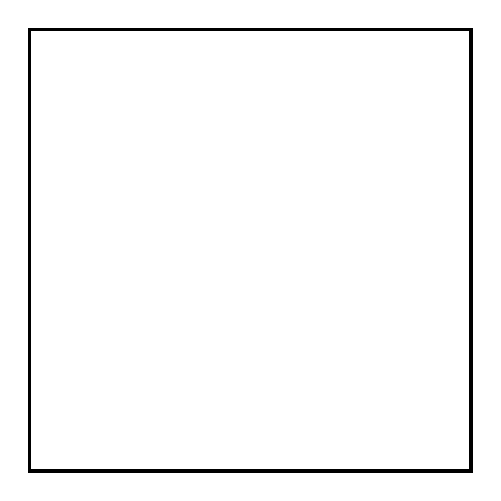
\begin{tikzpicture}
[borderdecorate/.style={-,very thick}]
%% chessboard with a black knight
\node at (0,4.9) {\WhiteEmptySquare\BlackEmptySquare\WhiteEmptySquare\BlackEmptySquare\WhiteEmptySquare\BlackEmptySquare\WhiteEmptySquare\BlackEmptySquare};
\node at (0,4.2) {\BlackEmptySquare\WhiteEmptySquare\BlackEmptySquare\WhiteEmptySquare\BlackEmptySquare\WhiteEmptySquare\BlackEmptySquare\WhiteEmptySquare};
\node at (0,3.5) {\WhiteEmptySquare\BlackEmptySquare\WhiteEmptySquare\BlackEmptySquare\WhiteEmptySquare\BlackEmptySquare\WhiteEmptySquare\BlackEmptySquare};
\node at (0,2.8) {\BlackEmptySquare\WhiteEmptySquare\BlackEmptySquare\WhiteEmptySquare\BlackKnightOnBlack\WhiteEmptySquare\BlackEmptySquare\WhiteEmptySquare};
\node at (0,2.1) {\WhiteEmptySquare\BlackEmptySquare\WhiteEmptySquare\BlackEmptySquare\WhiteEmptySquare\BlackEmptySquare\WhiteEmptySquare\BlackEmptySquare};
\node at (0,1.4) {\BlackEmptySquare\WhiteEmptySquare\BlackEmptySquare\WhiteEmptySquare\BlackEmptySquare\WhiteEmptySquare\BlackEmptySquare\WhiteEmptySquare};
\node at (0,0.7) {\WhiteEmptySquare\BlackEmptySquare\WhiteEmptySquare\BlackEmptySquare\WhiteEmptySquare\BlackEmptySquare\WhiteEmptySquare\BlackEmptySquare};
\node at (0,0.0) {\BlackEmptySquare\WhiteEmptySquare\BlackEmptySquare\WhiteEmptySquare\BlackEmptySquare\WhiteEmptySquare\BlackEmptySquare\WhiteEmptySquare};
%% the boarders of the chessboard
\draw[borderdecorate]
(-2.8,-0.352) -- (-2.8,5.257) -- (2.809,5.257) -- (2.809,-0.352) -- cycle;
\end{tikzpicture}
}
\quad
%%
%% knight's tour
\subfigure[A knight's tour.]{
\label{fig:graph_algorithms:one_knight_tour:a_tour}
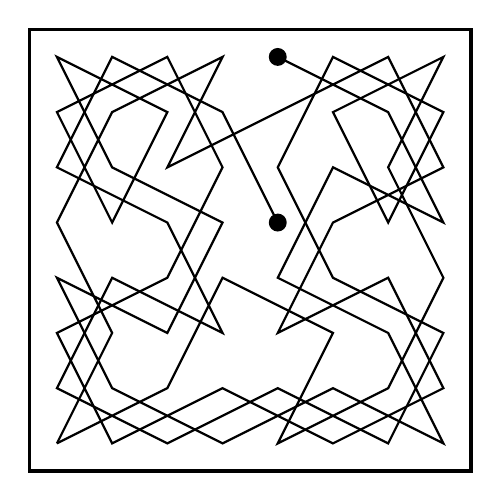
\begin{tikzpicture}
[borderdecorate/.style={-,very thick},%
  linedecorate/.style={-,thick},%
  nodedecorate/.style={shape=circle,fill=black,inner sep=2pt,draw,thick}]
%% empty chessboard
\node at (0,4.9) {\WhiteEmptySquare\BlackEmptySquare\WhiteEmptySquare\BlackEmptySquare\WhiteEmptySquare\BlackEmptySquare\WhiteEmptySquare\BlackEmptySquare};
\node at (0,4.2) {\BlackEmptySquare\WhiteEmptySquare\BlackEmptySquare\WhiteEmptySquare\BlackEmptySquare\WhiteEmptySquare\BlackEmptySquare\WhiteEmptySquare};
\node at (0,3.5) {\WhiteEmptySquare\BlackEmptySquare\WhiteEmptySquare\BlackEmptySquare\WhiteEmptySquare\BlackEmptySquare\WhiteEmptySquare\BlackEmptySquare};
\node at (0,2.8) {\BlackEmptySquare\WhiteEmptySquare\BlackEmptySquare\WhiteEmptySquare\BlackEmptySquare\WhiteEmptySquare\BlackEmptySquare\WhiteEmptySquare};
\node at (0,2.1) {\WhiteEmptySquare\BlackEmptySquare\WhiteEmptySquare\BlackEmptySquare\WhiteEmptySquare\BlackEmptySquare\WhiteEmptySquare\BlackEmptySquare};
\node at (0,1.4) {\BlackEmptySquare\WhiteEmptySquare\BlackEmptySquare\WhiteEmptySquare\BlackEmptySquare\WhiteEmptySquare\BlackEmptySquare\WhiteEmptySquare};
\node at (0,0.7) {\WhiteEmptySquare\BlackEmptySquare\WhiteEmptySquare\BlackEmptySquare\WhiteEmptySquare\BlackEmptySquare\WhiteEmptySquare\BlackEmptySquare};
\node at (0,0.0) {\BlackEmptySquare\WhiteEmptySquare\BlackEmptySquare\WhiteEmptySquare\BlackEmptySquare\WhiteEmptySquare\BlackEmptySquare\WhiteEmptySquare};
%% boarders of the chessboard
\draw[borderdecorate]
(-2.8,-0.352) -- (-2.8,5.257) -- (2.809,5.257) -- (2.809,-0.352) -- cycle;
%% map out knight's tour
\draw[linedecorate]
(-2.4494375,-0.0014374) -- ++(0.701125,1.40225) -- ++(-0.701125,1.40225)
-- ++(0.701125,1.40225) -- ++(1.40225,0.701125) -- ++(-0.701125,-1.40225)
-- ++(2.8045,1.40225) -- ++(0.701125,-1.40225) -- ++(-1.40225,-0.701125)
-- ++(-0.701125,-1.40225) -- ++(1.40225,0.701125) -- ++(0.701125,-1.40225)
-- ++(-1.40225,-0.701125) -- ++(-1.40225,0.701125) -- ++(-1.40225,-0.701125)
-- ++(-0.701125,1.40225) -- ++(1.40225,0.701125) -- ++(0.701125,1.40225)
-- ++(-0.701125,1.40225) -- ++(-1.40225,-0.701125) -- ++(0.701125,-1.40225)
-- ++(0.701125,1.40225) -- ++(-1.40225,0.701125) -- ++(0.701125,-1.40225)
-- ++(1.40225,-0.701125) -- ++(-0.701125,-1.40225) -- ++(-1.40225,0.701125)
-- ++(0.701125,-1.40225) -- ++(1.40225,-0.701125) -- ++(1.40225,0.701125)
-- ++(1.40225,-0.701125) -- ++(-0.701125,1.40225) -- ++(-1.40225,0.701125)
-- ++(0.701125,1.40225) -- ++(1.40225,-0.701125) -- ++(-0.701125,1.40225)
-- ++(-1.40225,0.701125);
\draw[linedecorate]
(-2.4494375,-0.0014374) -- ++(1.40225,0.701125) -- ++(0.701125,1.40225)
-- ++(1.40225,-0.701125) -- ++(-0.701125,-1.40225) -- ++(1.40225,0.701125)
-- ++(0.701125,1.40225) -- ++(-0.701125,1.40225) -- ++(0.701125,1.40225)
-- ++(-1.40225,-0.701125) -- ++(0.701125,-1.40225) -- ++(0.701125,1.40225)
-- ++(-1.40225,0.701125) -- ++(-0.701125,-1.40225) -- ++(0.701125,-1.40225)
-- ++(1.40225,-0.701125) -- ++(-0.701125,-1.40225) -- ++(-1.40225,0.701125)
-- ++(-1.40225,-0.701125) -- ++(-1.40225,0.701125) -- ++(0.701125,1.40225)
-- ++(1.40225,-0.701125) -- ++(-0.701125,1.40225) -- ++(-1.40225,0.701125)
-- ++(0.701125,1.40225) -- ++(1.40225,-0.701125) -- ++(0.701125,-1.40225);
%% filled dots to indicate the endpoints of the tour
\node at (0.3550625,2.8030626) [nodedecorate] {};
\node at (0.3550625,4.9064376) [nodedecorate] {};
\end{tikzpicture}
}
%%
%% graph representation of a knight's tour
\subfigure[Graph representation of tour.]{
\label{fig:graph_algorithms:one_knight_tour:graph_representation}
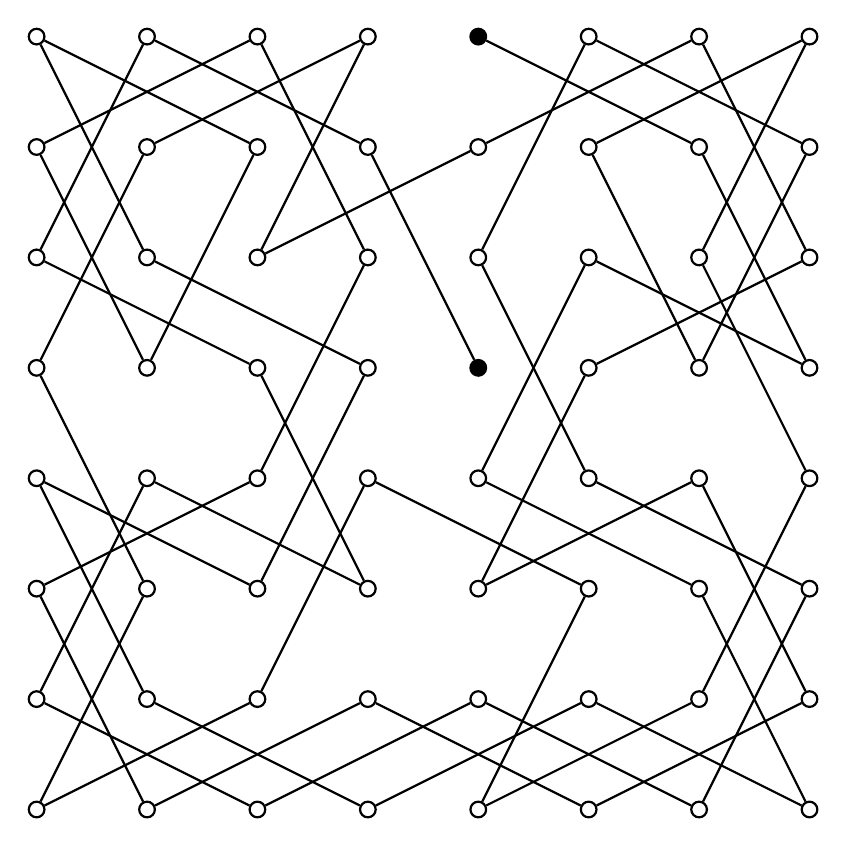
\begin{tikzpicture}
[linedecorate/.style={-,thick},%
  nodedecorate/.style={shape=circle,inner sep=2pt,draw,thick},%
  endpointdecorate/.style={shape=circle,fill=black,inner sep=2pt,draw,thick},%
  scale=2]
%% vertices or nodes
%% The coordinates of the chessboard are structured according to this
%% format
%%
%% 8
%% 7
%% *
%% *
%% *
%% 2
%% 1
%%   a  b  * * *  g  h
\foreach \nodename/\x/\y in {
a8/0/4.907875, b8/0.701125/4.907875, c8/1.40225/4.907875, d8/2.103375/4.907875, f8/3.505625/4.907875, g8/4.20675/4.907875, h8/4.907875/4.907875,
a7/0/4.20675, b7/0.701125/4.20675, c7/1.40225/4.20675, d7/2.103375/4.20675, e7/2.8045/4.20675, f7/3.505625/4.20675, g7/4.20675/4.20675, h7/4.907875/4.20675,
a6/0/3.505625, b6/0.701125/3.505625, c6/1.40225/3.505625, d6/2.103375/3.505625, e6/2.8045/3.505625, f6/3.505625/3.505625, g6/4.20675/3.505625, h6/4.907875/3.505625,
a5/0/2.8045, b5/0.701125/2.8045, c5/1.40225/2.8045, d5/2.103375/2.8045, f5/3.505625/2.8045, g5/4.20675/2.8045, h5/4.907875/2.8045,
a4/0/2.103375, b4/0.701125/2.103375, c4/1.40225/2.103375, d4/2.103375/2.103375, e4/2.8045/2.103375, f4/3.505625/2.103375, g4/4.20675/2.103375, h4/4.907875/2.103375,
a3/0/1.40225, b3/0.701125/1.40225, c3/1.40225/1.40225, d3/2.103375/1.40225, e3/2.8045/1.40225, f3/3.505625/1.40225, g3/4.20675/1.40225, h3/4.907875/1.40225,
a2/0/0.701125, b2/0.701125/0.701125, c2/1.40225/0.701125, d2/2.103375/0.701125, e2/2.8045/0.701125, f2/3.505625/0.701125, g2/4.20675/0.701125, h2/4.907875/0.701125,
a1/0/0, b1/0.701125/0, c1/1.40225/0, d1/2.103375/0, e1/2.8045/0, f1/3.505625/0, g1/4.20675/0, h1/4.907875/0}
{
  \node (\nodename) at (\x,\y) [nodedecorate] {};
}
%% endpoints of tour
\foreach \nodename/\x/\y in {e8/2.8045/4.907875, e5/2.8045/2.8045} {
  \node (\nodename) at (\x,\y) [endpointdecorate] {};
}
%% edges or lines
\path
\foreach \startnode/\endnode in {
e8/g7, g7/h5, h5/f6, f6/e4, e4/g3, g3/h1, h1/f2, f2/d1, d1/b2, b2/a4, a4/c3,
c3/d5, d5/b6, b6/a8, a8/c7, c7/b5, b5/a7, a7/c8, c8/d6, d6/c4, c4/a3, a3/b1,
b1/d2, d2/f1, f1/h2, h2/g4, g4/e3, e3/f5, f5/h6, h6/g8, g8/e7, e7/c6, c6/d8,
d8/b7, b7/a5, a5/b3, b3/a1, a1/c2, c2/d4, d4/f3, f3/e1, e1/g2, g2/h4, h4/g6,
g6/h8, h8/f7, f7/g5, g5/h7, h7/f8, f8/e6, e6/f4, f4/h3, h3/g1, g1/e2, e2/c1,
c1/a2, a2/b4, b4/d3, d3/c5, c5/a6, a6/b8, b8/d7, d7/e5}
{
  (\startnode) edge[linedecorate] node {} (\endnode)
};
\end{tikzpicture}
}
